% -*- root: ../ex6.tex -*-

\subsection{Bottlenecks and optimization} % (fold)
\label{sub:bottlenecks_and_optimization}

In our solver the root prosess has a lot of responsibilities. It is responsible for initializing the data, distributing it across all the other prosesses, collecting the data, and doing all of the transposes. This introduces a potential bottleneck in the solver depending on how large a problem size you want to run on it. 

Because all the network flow has to pass through our root node latency is expected to be larger than if every node arranged its own data for a collective distribution to all the other nodes through \texttt{MIP_Alltoallv}. Our reason for doing it this way is that we felt this approach had less complexity involved, and it was still possible to achieve a reasonable speedup. We timed each part of the serial version of \texttt{poission2D} and saw that the transpose operation used minimal time compoared to \emph{FST}. 

There are two possible improvements that can be done here. If you need to be able to solve larger tasks it would be advised to do the transpose in the \texttt{MPI_Send/MPI_Recv} itself. This could be achieved by the sender passing its columns to the reciever, and the reciever saving them as rows in its own matrix. As every prosessor has access to the \texttt{displacements} array it could easily place the recieved data from the other prosesses in the right place. This solution expects that all the recievers have a full $(N-1)\times(N-1)$ matrix in memory to be able to recieve whole rows/columns. In our solver, this would be the easiest change to make for a better speedup as the root prosess could save the recieved columns as rows. 

The other possible improvement is to make every prosess responsible for distributing its own data to all the other prosesses. As every prosess has access to the \texttt{partlens} they would all be aware of how much data is going to be sent/recieved by all the other prosesses. This could be implemented in the same fashion as mentioned earlier with every prosess having its own matrix in memory, or by a more complex solution where every process only recieves the data it expects (parts of columns from other prosesses) and nothing else, but this requires more complex code. The more complex solution would open for less memory usage as every prosess would not need to have the full matrix in memory. 

% Include figure matrix_blocktranspose.pdf
\begin{figure}[htbp]
	\centering
	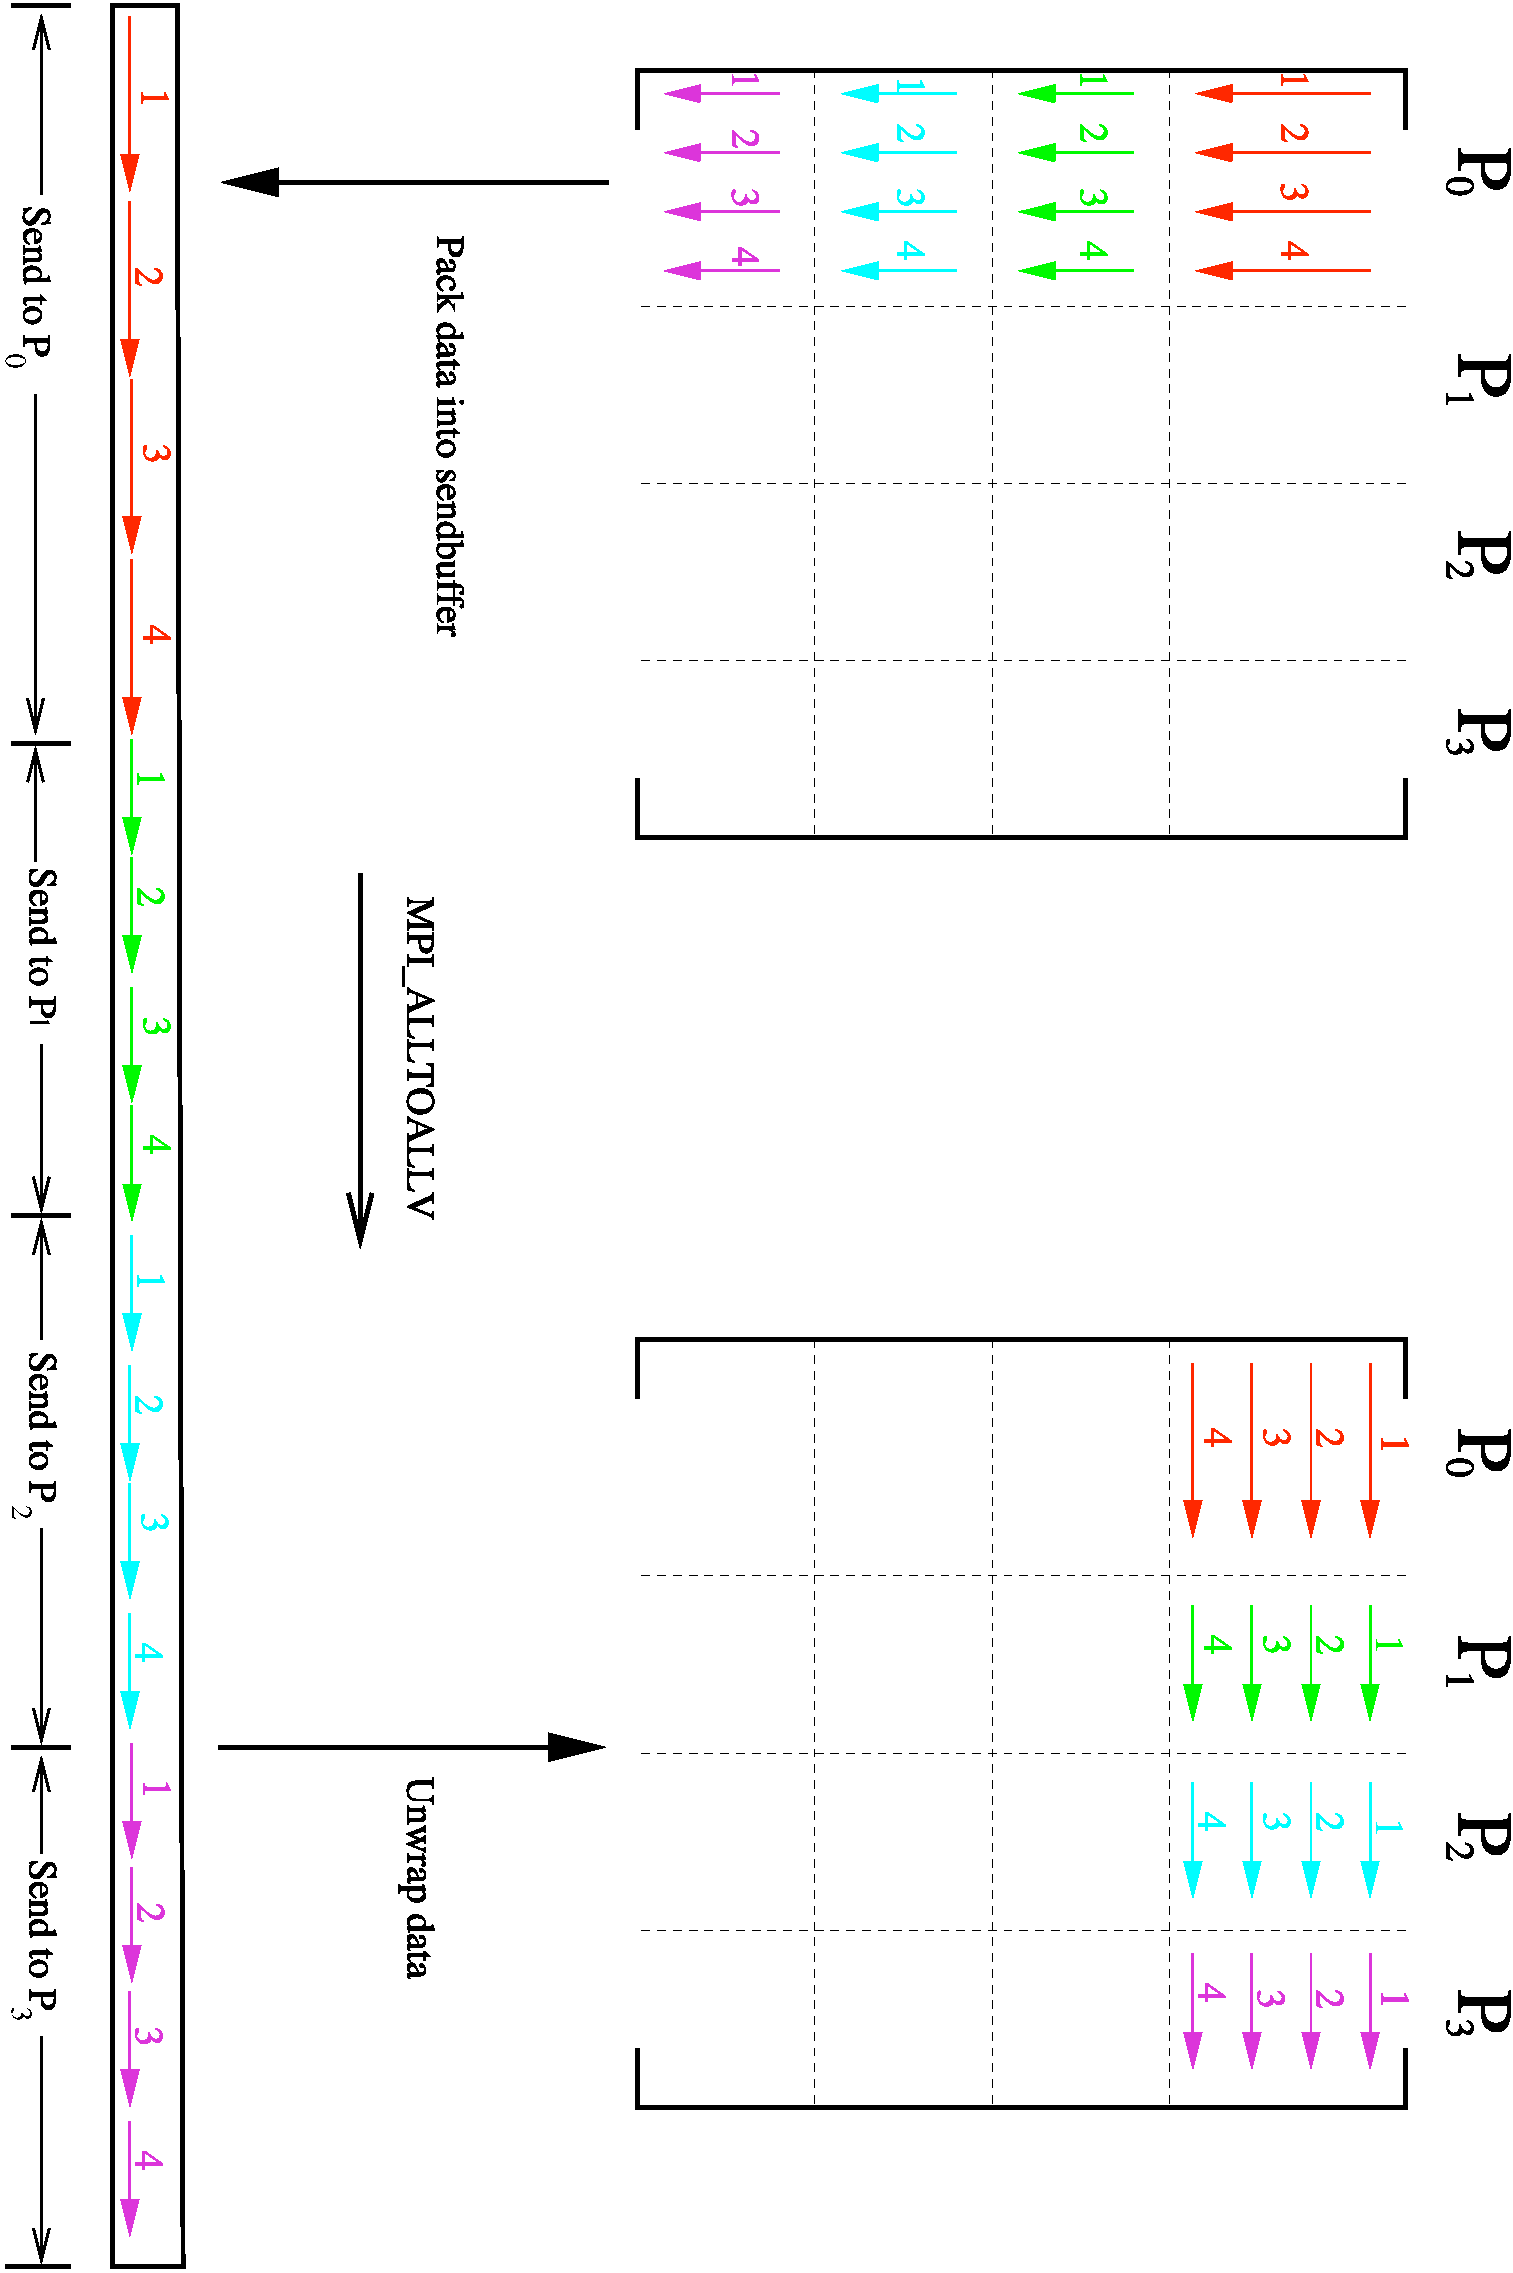
\includegraphics[width=0.95\textwidth]{illustrations/matrix_blocktranspose.pdf}
	\caption{The transpose operation using message passing: the packing and unpacking
of data. The figure is due to Bjarte Hægland.}
	\label{fig:label}
\end{figure}

This would also open the possibility to include the root prosess in more calculations as it's mainly used for organizing the solver and I/O.





% subsection bottlenecks_and_optimization (end)